\documentclass[10pt,a4paper]{article}
\usepackage[utf8]{inputenc}
\usepackage[german]{babel}
\usepackage{mathrsfs}
\usepackage{amsmath}
\usepackage{amsfonts}
\usepackage{amssymb}
\usepackage{amsthm}
\usepackage[left=2cm,right=2cm,top=2cm,bottom=2cm]{geometry}
\usepackage{graphicx}

\begin{document}

\section{Aufgabe 11}

Die ersten Stützstellen sind
\begin{equation}
  (0, \frac{1}{2}), (1, 1)
\end{equation}
Die Tschebyscheff-Stützstellen sind
\begin{equation}
  (\bar{x}_{1}, \frac{2 \sqrt{2}}{3 \sqrt{2} + 1}), (\bar{x}_{2}, \frac{2 \sqrt{2}}{3 \sqrt{2} - 1})
\end{equation}

Gesucht sind die Polynome
\begin{equation}
  f_{1}(x) = a_{2}x + a_{1}
\end{equation}
\begin{equation}
  f_{t}(x) = a_{4}x + a_{3}
\end{equation}

Die Gleichungssysteme sind
\begin{equation}
  \begin{pmatrix}
    1 & 0\\
    1 & 1
  \end{pmatrix}
  \cdot
  \begin{pmatrix}
    a_{1}\\a_{2}
  \end{pmatrix}
  =
  \begin{pmatrix}
    \frac{1}{2}\\
    1
  \end{pmatrix}
\end{equation}
\begin{equation}
  \begin{pmatrix}
    1 & \frac{1}{2} \left( 1 - \frac{1}{\sqrt{2}} \right)\\
    1 & \frac{1}{2} \left( 1 + \frac{1}{\sqrt{2}} \right)
  \end{pmatrix}
  \cdot
  \begin{pmatrix}
    a_{3}\\a_{4}
  \end{pmatrix}
  =
  \begin{pmatrix}
    \frac{2 \sqrt{2}}{3 \sqrt{2} + 1}\\
    \frac{2 \sqrt{2}}{3 \sqrt{2} - 1}
  \end{pmatrix}
\end{equation}

\begin{align*}
  & \frac{1}{\sqrt{2}}a_{4} = \frac{2 \sqrt{2}}{3 \sqrt{2} - 1} - \frac{2 \sqrt{2}}{3 \sqrt{2} + 1}\\
  \Leftrightarrow & \frac{1}{\sqrt{2}}a_{4} = \frac{2 \sqrt{2}((3 \sqrt{2} + 1) - (3 \sqrt{2} - 1))}{17} = \frac{4 \sqrt{2}}{17}\\
  \Leftrightarrow & a_{4} = \frac{8}{17}
\end{align*}
\begin{align*}
  a_{3} & = \frac{2 \sqrt{2}}{3 \sqrt{2} - 1} - \frac{1}{2} \left( 1 + \frac{1}{\sqrt{2}} \right) \frac{8}{17}\\
  & = \frac{2 \sqrt{2}}{3 \sqrt{2} - 1} - \frac{4}{17} \left( 1 + \frac{1}{\sqrt{2}} \right)\\
  & = \frac{2 \sqrt{2}}{3 \sqrt{2} - 1} - \frac{4 (1 + \sqrt{2})}{17 \sqrt{2}}\\
  & = \frac{2 \sqrt{2}}{3 \sqrt{2} - 1} - \frac{2 \sqrt{2} (1 + \sqrt{2})}{17}\\
  & = \frac{2 \sqrt{2}}{3 \sqrt{2} - 1} - \frac{2 \sqrt{2} + 4}{17}\\
  & = \frac{17 \cdot 2 \sqrt{2} - (3 \sqrt{2} - 1)(2 \sqrt{2} + 4)}{17 (3 \sqrt{2} - 1)}\\
  & = \frac{34 \sqrt{2} - 12 - 12 \sqrt{2} + 2 \sqrt{2} + 4}{17 (3 \sqrt{2} - 1)}\\
  & = \frac{24 \sqrt{2} - 8}{17 (3 \sqrt{2} - 1)}\\
\end{align*}

Also sind
\begin{equation}
  f_{1}(x) = \frac{1}{2}x + \frac{1}{2}
\end{equation}
\begin{equation}
  f_{t}(x) = \frac{4}{3\sqrt{2} + 1}x + \frac{24 \sqrt{2} - 8}{17 (3 \sqrt{2} - 1)}
\end{equation}

\begin{equation}
  f'(x) = \frac{1}{(2 - x)^{2}}
\end{equation}
\begin{equation}
  f''(x) = \frac{2}{(2 - x)^{3}}
\end{equation}
\begin{equation}
  f'''(x) = \frac{6}{(2 - x)^{4}}
\end{equation}
\begin{equation}
  |f''|_{\infty, [0, 1]} = f''(1) = 2 \textit{weil $f'''(x) > 0$ für $x \in [0, 1]$}
\end{equation}

Die Fehlerabschätzungen sind
\begin{equation}
  \max_{x \in [0, 1]} |f(x) - f_{1}(x)| \le \max_{x \in [0, 1]} \frac{2}{2} |x| \cdot |x - 1| = \frac{1}{4}
\end{equation}
\begin{align*}
  \max_{x \in [0, 1]} |f(x) - f_{t}(x)| & \le \max_{x \in [0, 1]} |x - \frac{2 \sqrt{2}}{3 \sqrt{2} + 1}| \cdot |x - \frac{2 \sqrt{2}}{3 \sqrt{2} - 1}|\\
  & = \max_{x \in [0, 1]} |x^{2} - (\frac{2 \sqrt{2}}{3 \sqrt{2} + 1} + \frac{2 \sqrt{2}}{3 \sqrt{2} - 1})x + \frac{2 \sqrt{2}}{3 \sqrt{2} + 1}\frac{2 \sqrt{2}}{3 \sqrt{2} - 1}|\\
  & = \max_{x \in [0, 1]} |x^{2} - \frac{24}{17}x + \frac{8}{17}| \textit{ Extremum bei $x = \frac{12}{17}$}\\
  & = \max_{x \in [0, 1]} \{ \frac{8}{17}, \frac{1}{17}, \frac{52}{289} \} \textit{ Werte für $0$, $1$, $\frac{12}{17}$}\\
  & = \frac{8}{17}
\end{align*}

\subsection{Der tatsächliche Fehler im ersten Fall}

\begin{equation}
  q(x) = f(x) - f_{1}(x) = \frac{1}{2 - x} - \frac{1}{2}x - \frac{1}{2}
\end{equation}
\begin{equation}
  q'(x) = \frac{1}{(2 - x)^{2}} - \frac{1}{2}
\end{equation}
\begin{equation}
  q'(x) = 0 \Leftrightarrow \frac{1}{(2 - x)^{2}} = \frac{1}{2} \Leftrightarrow (2 - x)\frac{1}{\sqrt{2}} = 1 \Leftrightarrow x = 2 - \sqrt{2}
\end{equation}
Dies muss betragsmäßig das Maximum sein, weil die Randwerte wegen der Interpolationsbedingung beide $0$ sind.
\begin{equation}
  \max_{\infty, [0, 1]} |q(x)| = |\frac{1}{\sqrt{2}} - 1 + \frac{1}{\sqrt{2}} - \frac{1}{2}| = |\frac{2}{\sqrt{2}} - \frac{3}{2}| = |\sqrt{2} - \frac{3}{2}| \approx 0.09
\end{equation}

\subsection{Der tatsächliche Fehler im zweiten Fall}

\begin{equation}
  q(x) = f(x) - f_{t}(x) = \frac{1}{2 - x} - \frac{4}{3\sqrt{2} + 1}x - \frac{24 \sqrt{2} - 8}{17 (3 \sqrt{2} - 1)}
\end{equation}
\begin{equation}
  q'(x) = \frac{1}{(2 - x)^{2}} - \frac{4}{3\sqrt{2} + 1}
\end{equation}
\begin{align*}
  q'(x) = 0 \Leftrightarrow & \frac{1}{(2 - x)^{2}} = \frac{4}{3\sqrt{2} + 1}\\
  \Leftrightarrow & \frac{1}{2 - x} = \frac{2}{\sqrt{3\sqrt{2} + 1}}\\
  \Leftrightarrow & \frac{2}{\sqrt{3\sqrt{2} + 1}}(2 - x) = 1\\
  \Leftrightarrow & \frac{4}{\sqrt{3\sqrt{2} + 1}} - \frac{2x}{\sqrt{3\sqrt{2} + 1}} = 1\\
  \Leftrightarrow & \frac{4}{\sqrt{3\sqrt{2} + 1}} - 1 = \frac{2x}{\sqrt{3\sqrt{2} + 1}}\\
  \Leftrightarrow & x = \frac{4}{\sqrt{3\sqrt{2} + 1}}\frac{\sqrt{3\sqrt{2} + 1}}{2} - \frac{\sqrt{3\sqrt{2} + 1}}{2} = 2 - \frac{\sqrt{3\sqrt{2} + 1}}{2}
\end{align*}
$q$ hat an dieser Stelle den Wert
\begin{align*}
  q(2 - \frac{\sqrt{3\sqrt{2} + 1}}{2}) & = \frac{1}{\frac{\sqrt{3\sqrt{2} + 1}}{2}} - \frac{4}{3\sqrt{2} + 1}(2 - \frac{\sqrt{3\sqrt{2} + 1}}{2}) - \frac{24 \sqrt{2} - 8}{17 (3 \sqrt{2} - 1)}\\
  & = \frac{2}{\sqrt{3\sqrt{2} + 1}} - \frac{8}{3\sqrt{2} + 1} + \frac{2}{\sqrt{3\sqrt{2} + 1}} - \frac{24 \sqrt{2} - 8}{17 (3 \sqrt{2} - 1)}\\
  & = \frac{4}{\sqrt{3\sqrt{2} + 1}} - \frac{8}{3\sqrt{2} + 1} - \frac{24 \sqrt{2} - 8}{17 (3 \sqrt{2} - 1)}\\
  & = \frac{4 \sqrt{3\sqrt{2} + 1} - 8}{3\sqrt{2} + 1} - \frac{24 \sqrt{2} - 8}{17 (3 \sqrt{2} - 1)}\\
  & = \frac{(17 (3 \sqrt{2} - 1))(4 \sqrt{3\sqrt{2} + 1} - 8) - (3\sqrt{2} + 1)(24 \sqrt{2} - 8)}{17^{2}}\\
  & = \frac{(51 \sqrt{2} - 17)(4 \sqrt{3\sqrt{2} + 1} - 8) - (144 - 24\sqrt{2} + 24 \sqrt{2} - 8)}{17^{2}}\\
  & = \frac{(204\sqrt{2}\sqrt{3\sqrt{2} + 1} - 408\sqrt{2} - 68\sqrt{3\sqrt{2} + 1} + 136) - 136}{17^{2}}\\
  & = \frac{204\sqrt{2}\sqrt{3\sqrt{2} + 1} - 408\sqrt{2} - 68\sqrt{3\sqrt{2} + 1}}{17^{2}} \approx -0.25
\end{align*}
\begin{align*}
  \max_{\infty, [0, 1]} |q(x)| = \{ 0.25, |\frac{24 \sqrt{2} - 8}{17 (3 \sqrt{2} - 1)}|, |q(1)| \} \approx \max_{\infty, [0, 1]} |q(x)| = \{ 0.25, \frac{1}{34}, 0.23 \} = 0.25
\end{align*}

\section{Aufgabe 12}

\section{Aufgabe 13}

Die Stützstellen sind
\begin{equation}
  (-5, \frac{1}{26}), (-3, \frac{1}{10}), (-1, \frac{1}{2}), (1, \frac{1}{2}), (3, \frac{1}{10}), (5, \frac{1}{26})
\end{equation}
Dann ist das lineare Gleichungssystem
\begin{equation}
  \begin{pmatrix}
    2 & \frac{1}{2} & 0 & 0 & 0 & 0\\
    \frac{1}{2} & 2 & \frac{1}{2} & 0 & 0 & 0\\
    0 & \frac{1}{2} & 2 & \frac{1}{2} & 0 & 0\\
    0 & 0 & \frac{1}{2} & 2 & \frac{1}{2} & 0\\
    0 & 0 & 0 & \frac{1}{2} & 2 & \frac{1}{2}\\
    0 & 0 & 0 & 0 & \frac{1}{2} & 2
  \end{pmatrix}
  \cdot
  \begin{pmatrix}
    v_{1}\\
    v_{2}\\
    v_{3}\\
    v_{4}\\
    v_{5}\\
    v_{6}
  \end{pmatrix}
  =
  \frac{3}{4} \cdot
  \begin{pmatrix}
    \frac{1}{10}\\
    \frac{6}{13}\\
    \frac{2}{5}\\
    -\frac{2}{5}\\
    -\frac{6}{13}\\
    -\frac{1}{10}
  \end{pmatrix}
  =
  \begin{pmatrix}
    \frac{3}{40}\\
    \frac{9}{26}\\
    \frac{3}{10}\\
    -\frac{3}{10}\\
    -\frac{9}{26}\\
    -\frac{3}{40}
  \end{pmatrix}
\end{equation}

Die Lösung ist
\begin{equation}
  \begin{pmatrix}
    v_{1}\\
    v_{2}\\
    v_{3}\\
    v_{4}\\
    v_{5}\\
    v_{6}
  \end{pmatrix}
  =
  \begin{pmatrix}
    \frac{9}{2132}\\
    \frac{1419}{10660}\\
    \frac{1659}{10660}\\
    -\frac{1659}{10660}\\
    -\frac{1419}{10660}\\
    -\frac{9}{2132}
  \end{pmatrix}
\end{equation}

Die einzelnen Polynome sehen also wie folgt aus
\begin{align*}
  p_{1}(x) = & (1 - \frac{x + 5}{2}) \cdot \frac{1}{26} + \frac{x + 5}{2} \cdot \frac{1}{10}\\
  & + \frac{x + 5}{2} \cdot (1 - \frac{x + 5}{2}) \cdot ((2 \cdot \frac{9}{2132} - (\frac{1}{10} - \frac{1}{26})) (1 - \frac{x + 5}{2})\\
  & + ((-2\frac{1419}{10660} + (\frac{1}{10} - \frac{1}{26}))) \cdot \frac{x + 5}{2})
\end{align*}

Die restlichen schreibe ich mal nicht aus.

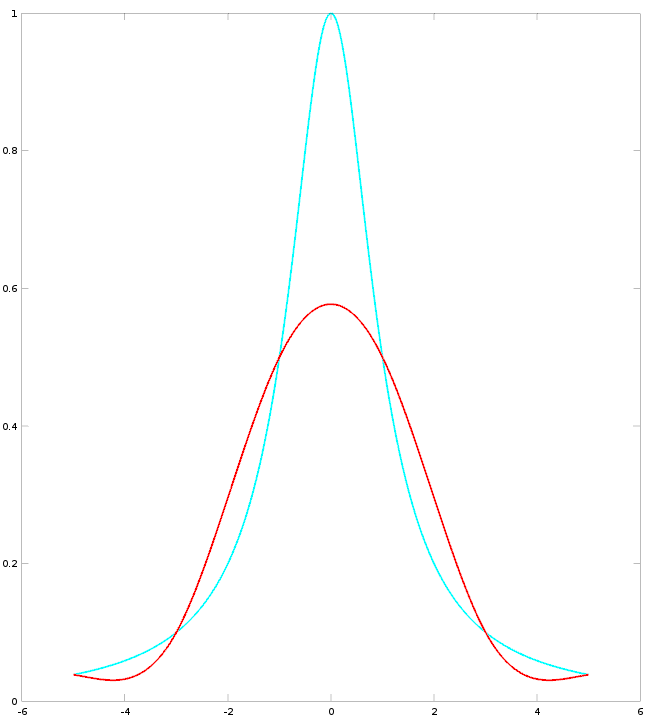
\includegraphics[width=300pt]{4_13.png}

\end{document}